\section{The Complete Standard Model, Successes and Shortcomings}
\label{sec:final_sm_description}

The physical field content of the SM, after EWSB, is detailed in Table~\ref{tab:sm_content_EWSB}
Also shown in Table~\ref{tab:sm_content_EWSB} are the electric charge associated with each
particle field, $Q$, the relevant couplings, and particle masses.


\begin{table}[!htb]
    \caption{
        The particle content of the SM after the process of
        electroweak symmetry breaking.
    }
    \begin{center}
        \begin{tabularx}{1\textwidth}{m{1em} c c c c }
        \toprule
        \hline
        & Physical Field & Q & Coupling & Mass [GeV] \\
        \hline
        \rotatebox{90}{\hspace{-0.1cm}\textbf{Quarks} } 
            & \makecell{ \quarkU, \quarkC, \quarkT \\ \quarkD, \quarkS, \quarkB} % FIELD
            & \makecell{ $2/3$ \\ $-1/3$ }% Q
            %& \makecell{ $\mathbf{3}$ \\ $\mathbf{3}$ } % SU(3)
            & \makecell{ ($y_i=$) $1\times10^{-5}$, $7\times10^{-3}$, $1$ \\ ($y_i=$) $3\times10^{-5}$, $5\times10^{-4}$, $0.02$ } % Coupling
            & \makecell{ $2\times10^{-3}$, $1.27$, $173$ \\ $4\times10^{-4}$, $0.10$, $4.18$ }\\% Mass
        \rotatebox{90}{\hspace{-0.1cm}\textbf{Leptons} } 
            & \makecell{ \leptonE, \leptonMu, \leptonTau \\ \neutrinoE, \neutrinoMu, \neutrinoTau } % FIELD
            & \makecell{ $-1$ \\ $0$ }% Q
            %& \makecell{ $\mathbf{1}$ \\ $\mathbf{1}$ } % SU(3)
            & \makecell{ ($y_i=$) $3\times10^{-7}$, $6\times10^{-4}$, $0.01$ \\ -- } % Coupling
            & \makecell{ $5\times10^{-4}$, $0.106$, $1.777$ \\ --}\\% Mass
        \midrule
        \rotatebox{90}{\textbf{Bosons} } 
            & \makecell{ \fieldPhoton \\ \fieldZ \\ (\fieldWp, \fieldWm) \\ \fieldG } % FIELD
            & \makecell{ $0$ \\ $0$ \\ $(+1,-1)$ \\ $0$ }% Q
            %& \makecell{ $\mathbf{1}$ \\ $\mathbf{1}$ \\ $\mathbf{1}$ \\ $\mathbf{8}$ } % SU(3)
            & \makecell{ $\alpha_{\text{EM}} \simeq 1/137$ \\ $\sin \theta_{W} \simeq 0.5$ \\ -- \\ $\alpha_s \simeq 0.1$ } % Coupling
            & \makecell{ $0$ \\ $91.2$ \\ $80.4$ \\  $0$}\\% Mass
        \midrule
        \rotatebox{90}{\textbf{Higgs} } 
            & \makecell{ \fieldH } % FIELD
            & \makecell{ $0$ }% Q
            %& \makecell{ $\mathbf{1}$ } % SU(3)
            & \makecell{ $\lambda$, $\mu$ } % Coupling
            & \makecell{ $125.09$ }\\% Mass

         %&   \makecell{ (\quarkUl, \quarkDl), (\quarkCl, \quarkSl), (\quarkTl, \quarkBl) \\ \quarkUr \\ \quarkDr}% CONTENT
         %&   \makecell{ $1/2$ \\ $1/2$ \\ $1/2$} % SPIN
         %&   \makecell{ $\mathbf{2}$ \\ $\mathbf{1}$ \\ $\mathbf{1}$}% SU(2)
         %&   \makecell{ $\mathbf{3}$ \\ $\mathbf{3}$ \\ $\mathbf{3}$}\\ % SU(3)
        %%\cdashline{1-7}
        %rotatebox{90}{\hspace{-0.1cm}\textbf{Leptons} }
         %&   \makecell{\quarkLi \\ \quarkEri} % FIELD
         %&   \makecell{ (\quarkEl, \quarkNuEl), (\quarkMul, \quarkNuMul), (\quarkTaul, \quarkNuTaul) \\ \quarkEr, \quarkMur, \quarkTaur}% CONTENT
         %&   \makecell{ $1/2$ \\ $1/2$ }% SPIN
         %&   \makecell{ $\mathbf{2}$ \\ $\mathbf{1}$ }% SU(2)
         %&   \makecell{ $\mathbf{1}$ \\ $\mathbf{1}$ } \\ % SU(3)
        %midrule
        %rotatebox{90}{\textbf{\stackanchor{Gauge}{Fields}} }
         %&   \makecell{\quarkB \\ \quarkW \\ \quarkG } % FIELD
         %&   \makecell{ \quarkB \\ (\quarkWone, \quarkWtwo, \quarkWthree) \\ \quarkG }% CONTENT
         %&   \makecell{ $1$ \\ $1$ \\ $1$} % SPIN
         %&   \makecell{ $\mathbf{1}$ \\ $\mathbf{3}$ \\ $\mathbf{1}$}% SU(2)
         %&   \makecell{ $\mathbf{1}$ \\ $\mathbf{1}$ \\ $\mathbf{8}$}\\ % SU(3)
        %midrule
        %rotatebox{90}{\textbf{\stackanchor{Higgs}{Field}}} 
         %&   \makecell{\quarkPhi } % FIELD
         %&   \makecell{ (\quarkPhip, \quarkPhizero) }% CONTENT
         %&   \makecell{ $0$  } % SPIN
         %&   \makecell{ $\mathbf{2}$ }% SU(2)
         %&   \makecell{ $\mathbf{1}$ }\\ % SU(3)
        \hline
        \bottomrule
        \end{tabularx}
    \end{center}
    \label{tab:sm_content}
\end{table}


%%%%%%%%%%%%%%%%%%%%%%%%%%%%%%%%%%%%%%%%%%%%%%%%%%%%%%%%%%%%%%%%%%%%%%%%%%%%%%%%%
%%%%%%%%%%%%%%%%%%%%%%%%%%%%%%%%%%%%%%%%%%%%%%%%%%%%%%%%%%%%%%%%%%%%%%%%%%%%%%%%%
%%%%%%%%%%%%%%%%%%%%%%%%%%%%%%%%%%%%%%%%%%%%%%%%%%%%%%%%%%%%%%%%%%%%%%%%%%%%%%%%%
%
% SUCCESSES
%
%%%%%%%%%%%%%%%%%%%%%%%%%%%%%%%%%%%%%%%%%%%%%%%%%%%%%%%%%%%%%%%%%%%%%%%%%%%%%%%%%
%%%%%%%%%%%%%%%%%%%%%%%%%%%%%%%%%%%%%%%%%%%%%%%%%%%%%%%%%%%%%%%%%%%%%%%%%%%%%%%%%
%%%%%%%%%%%%%%%%%%%%%%%%%%%%%%%%%%%%%%%%%%%%%%%%%%%%%%%%%%%%%%%%%%%%%%%%%%%%%%%%%

\subsection{Successes of the Standard Model}
\label{sec:sm_successes}

The particle content presented in Table~\ref{tab:sm_content_EWSB} represents the current
picture of the visible matter content of the universe.
It is a concise picture.
With this particle content in hand, and the description of their fundamental particle interactions (Equation~\ref{eq:sm_lagrangian}),
the predictive power of the SM is immense.

Figure~\ref{fig:sm_xsec_summary} shows a summary of LHC measurements of cross-sections
for various production processes at 7, 8, and 13\,TeV.
The agreement of these measurements with the theoretical predictions provided by the SM, spanning over 10 orders of magnitude,
is an incredible testament to the power of the SM and the toolkit provided by QFT.
The power of the SM, and its internal consistency, is illustrated in Figure~\ref{fig:mw_mt_scan},
which shows the results of indirect measurements of the $W$-boson and top-quark masses based
on fits to electroweak precision data.
When all measurements other than those on $m_h$ are included, the constraints of the SM
only allow for a small region of the $(m_{\text{top}}, M_W)$ parameter space.
Adding the Higgs measurements results only shrinks this allowed area.
The fact that these indirect measurements agree so well with the direct measurements paints a picture
of the SM as being a fundamentally complete picture of the known physical phenomena.
If the SM were not accounting for particular types of interactions or known fields,
the level of agreement between the direct measurements and those obtained indirectly via
fits to electroweak precision data would not be to the level seen in Figure~\ref{fig:mw_mt_scan}.

\begin{figure}[!htb]
    \begin{center}
        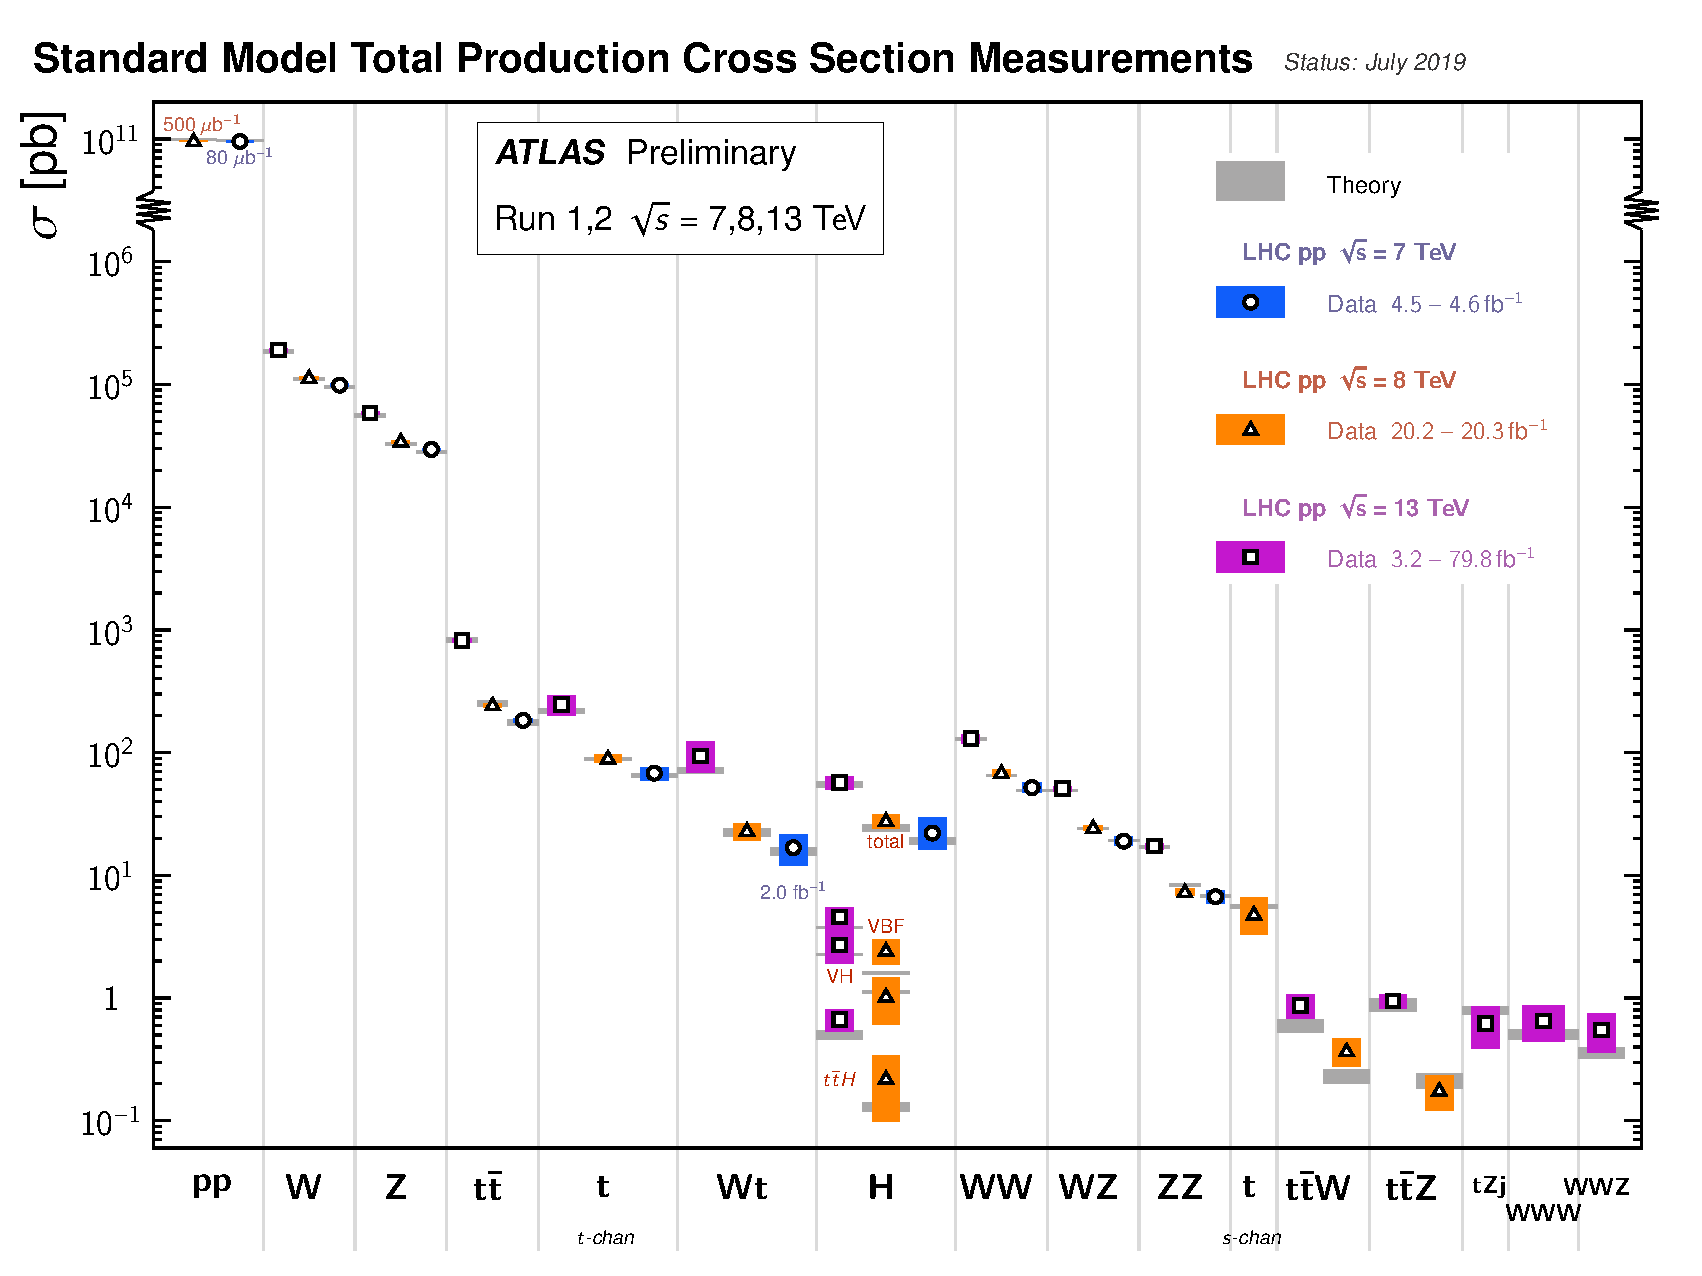
\includegraphics[width=0.75\textwidth]{figures/chapter1/sm_final/sm_xsec_summary}
        \caption{
            Summary of several Standard Model total production cross section measurements,
            corrected for branching fractions, compared to the corresponding theoretical expectations. 
        }
        \label{fig:sm_xsec_summary}
    \end{center}
\end{figure}
\begin{figure}[!htb]
    \begin{center}
        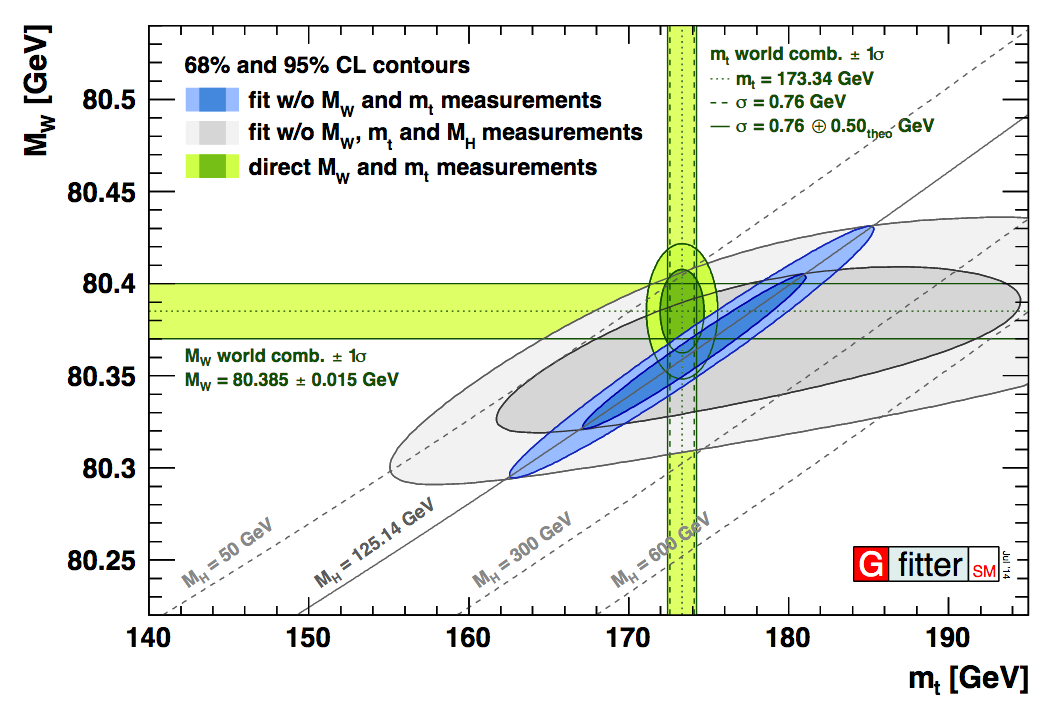
\includegraphics[width=0.75\textwidth]{figures/chapter1/sm_final/mw_vs_mt_indirect}
        \caption{
            Contours at 68\% and 95\% CL obtained from scans of $M_W$ versus $m_{\text{top}}$,
            for the global electroweak fit including the Higgs boson mass ($m_h$) measurements~\cite{HMassATLAS,HMassCMS} (blue)
            and excluding the $m_h$ measurements (grey), as compared t the direct
            measurements of these quantities (green bands and ellipses).
            From Ref.~\cite{GFitter}.
        }
        \label{fig:mw_mt_scan}
    \end{center}
\end{figure}

With the discovery a Higgs boson like particle with a mass at 125\,GeV in 2012~\cite{HDiscoveryATLAS,HDiscoveryCMS},
the final piece of the SM described by Equation~\ref{eq:sm_lagrangian} is potentially found.
The 2012 Higgs discovery meant the start of a very long experimental program began, focused
on studying this new particle and confirming its role as being the fundamental scalar boson, $\phi$,
appearing in Equation~\ref{eq:sm_lagrangian}.

It should be stressed that the terms associated with the Higgs potential appearing in the SM
Lagrangian, given by Equation~\ref{eq:higgs_potential}, are by no means fundamental.
They did (and do) not have to appear in this way.
The terms appearing in Equation~\ref{eq:higgs_potential} take the form they do since they
could lead to masses for the fermions and gauge bosons.
There is no fundamental symmetry motivating their form or appearance.
The BEH mechanism is inspired by the formation of composite (i.e. not elementary) scalar particles
appearing in super-conductivity (Cooper pairs).
The fact that the same type of phase transition should describe the generation of masses for
the elementary particles of the SM, and that it should presuppose the existence of an \textit{elementary}
scalar boson, was simply left as one of the last open questions of the SM.
In a sense, the truth of the form underlying Equation~\ref{eq:higgs_potential} was not important to BEH.
The more important takeaway was that there \textit{could} be a mechanism by which the SM particles acquired
mass without disrupting the gauge structure that had already held up to experimental scrutiny.
%In a certain sense, this is reflected by the fact that BEH were awarded the Nobel prize only \textit{after} the discoveries of the ATLAS and CMS experiments
%in 2012, whereas GWS were awarded theirs several years \textit{before} the experimental verification of
%the existence of the $W$ and $Z$ bosons.

It is then up to the experiments to verify that the 125\,GeV scalar boson discovered in 2012
is responsible for the BEH mechanism as described in Section~\ref{sec:higgs_description}.
The form of the Higgs potential as defined in Equation~\ref{eq:higgs_potential} makes
very clear predictions on the form and strengths of the couplings to the known fundamental particles:
the fermions and gauge bosons, with couplings to the Higgs predicted to take the forms
of Equations~\ref{eq:higgs_fermion_coupling} and \ref{eq:higgs_gauge_couplings}, respectively.
It is then up to the ATLAS and CMS experiments to verify that the new particle couples
to these `old' particles just as predicted.
The coupling strengths also dictate the Higgs decay rates into specific SM particles, as indicated
in Figure~\ref{fig:higgs_br_sm}.
Any deviation in the measured values of the SM-predicted Higgs decay branching ratios or
in the predicted values of the fermion or gauge coupling strengths, and their dependence on the
particle masses, would indicate that the particle discovered in 2012 is not the Higgs boson as predicted
in the SM.

All of the measurements of the properties of the 125 GeV particle
made by the ATLAS and CMS experiments are so far in fairly good agreement with the SM prediction
of a $m_h = 125$ GeV Higgs boson~\cite{HProp0,HProp1,HProp2,HProp3,HProp4,HProp5,HProp6,HProp7,HProp8}.
The agreement with the SM prediction, over a wide variety of measurements, is illustrated in
Figure~\ref{fig:higgs_measurements} which shows the measurements of the fermion and gauge
couplings and of the cross-sections of the leading Higgs production mechanisms and decay
branching ratios.
Within the precision of these measurements, the SM is fully supported by the experiments
and it appears as though the particle discovered in 2012 is in fact the particle as predicted
by BEH.

\begin{figure}[!htb]
    \begin{center}
        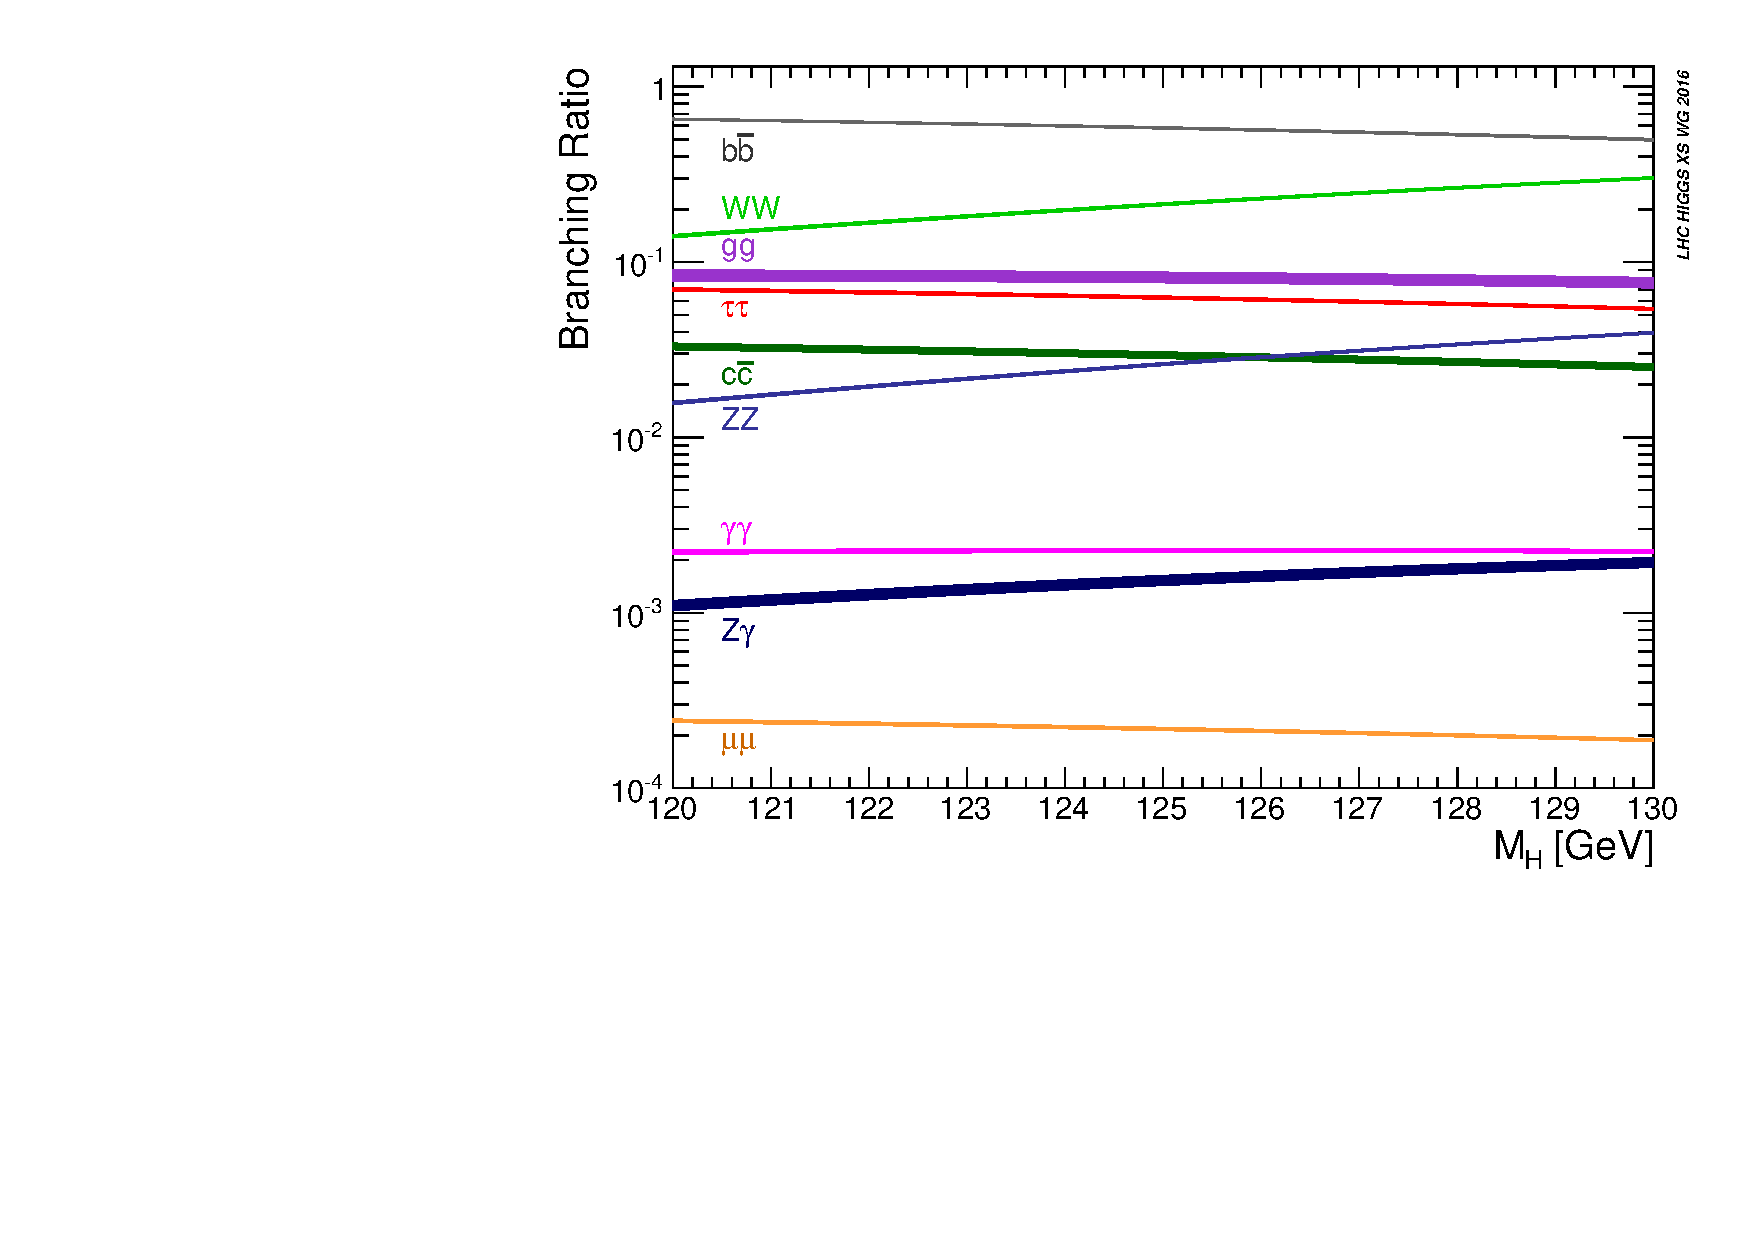
\includegraphics[width=0.6\textwidth]{figures/chapter1/sm_final/higgs_br_sm}
        \caption{
            Predicted branching ratios for an SM-like Higgs boson with $m_{h} = 125\,\GeV$.
        }
        \label{fig:higgs_br_sm}
    \end{center}
\end{figure}

\begin{figure}[!htb]
    \begin{center}
        \raisebox{1cm}{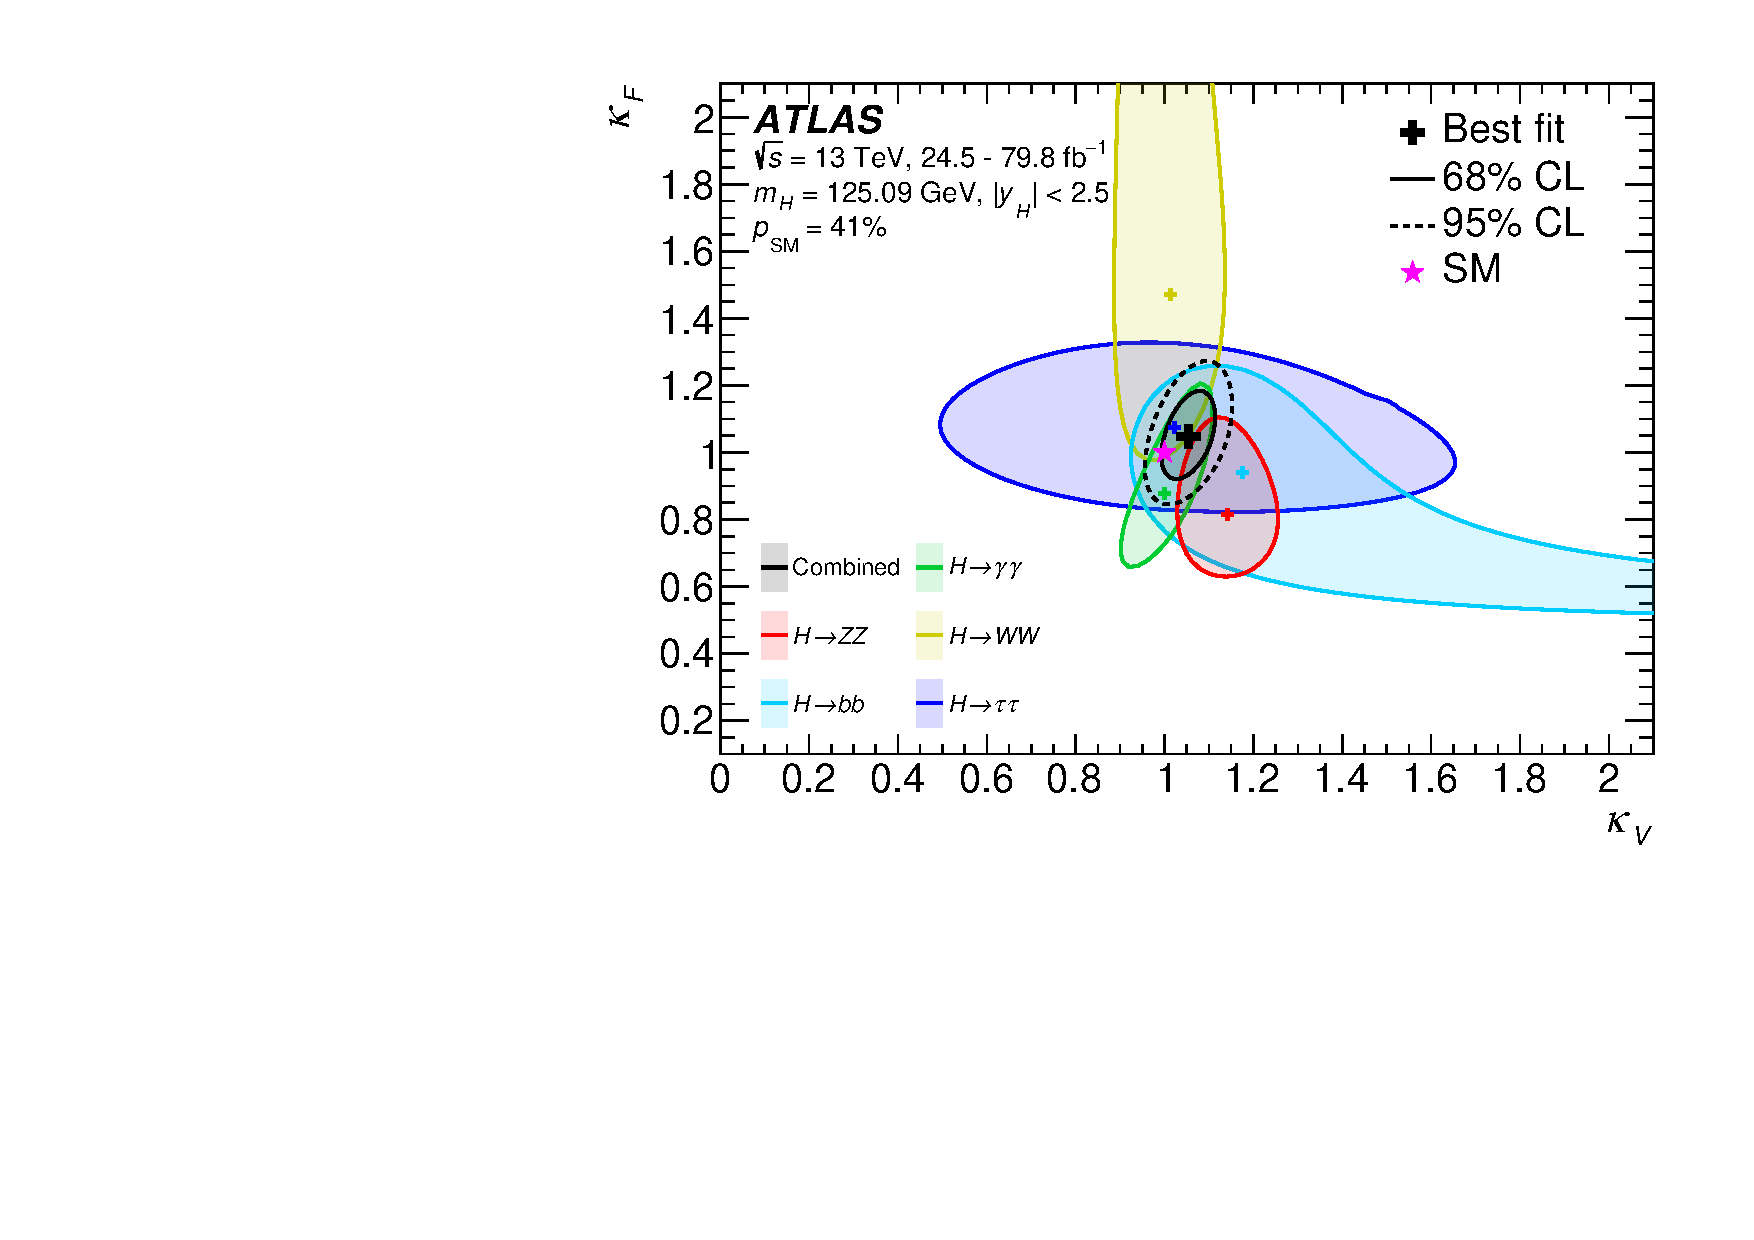
\includegraphics[width=0.49\textwidth]{figures/chapter1/sm_final/higgs_kappa_v_f}}
        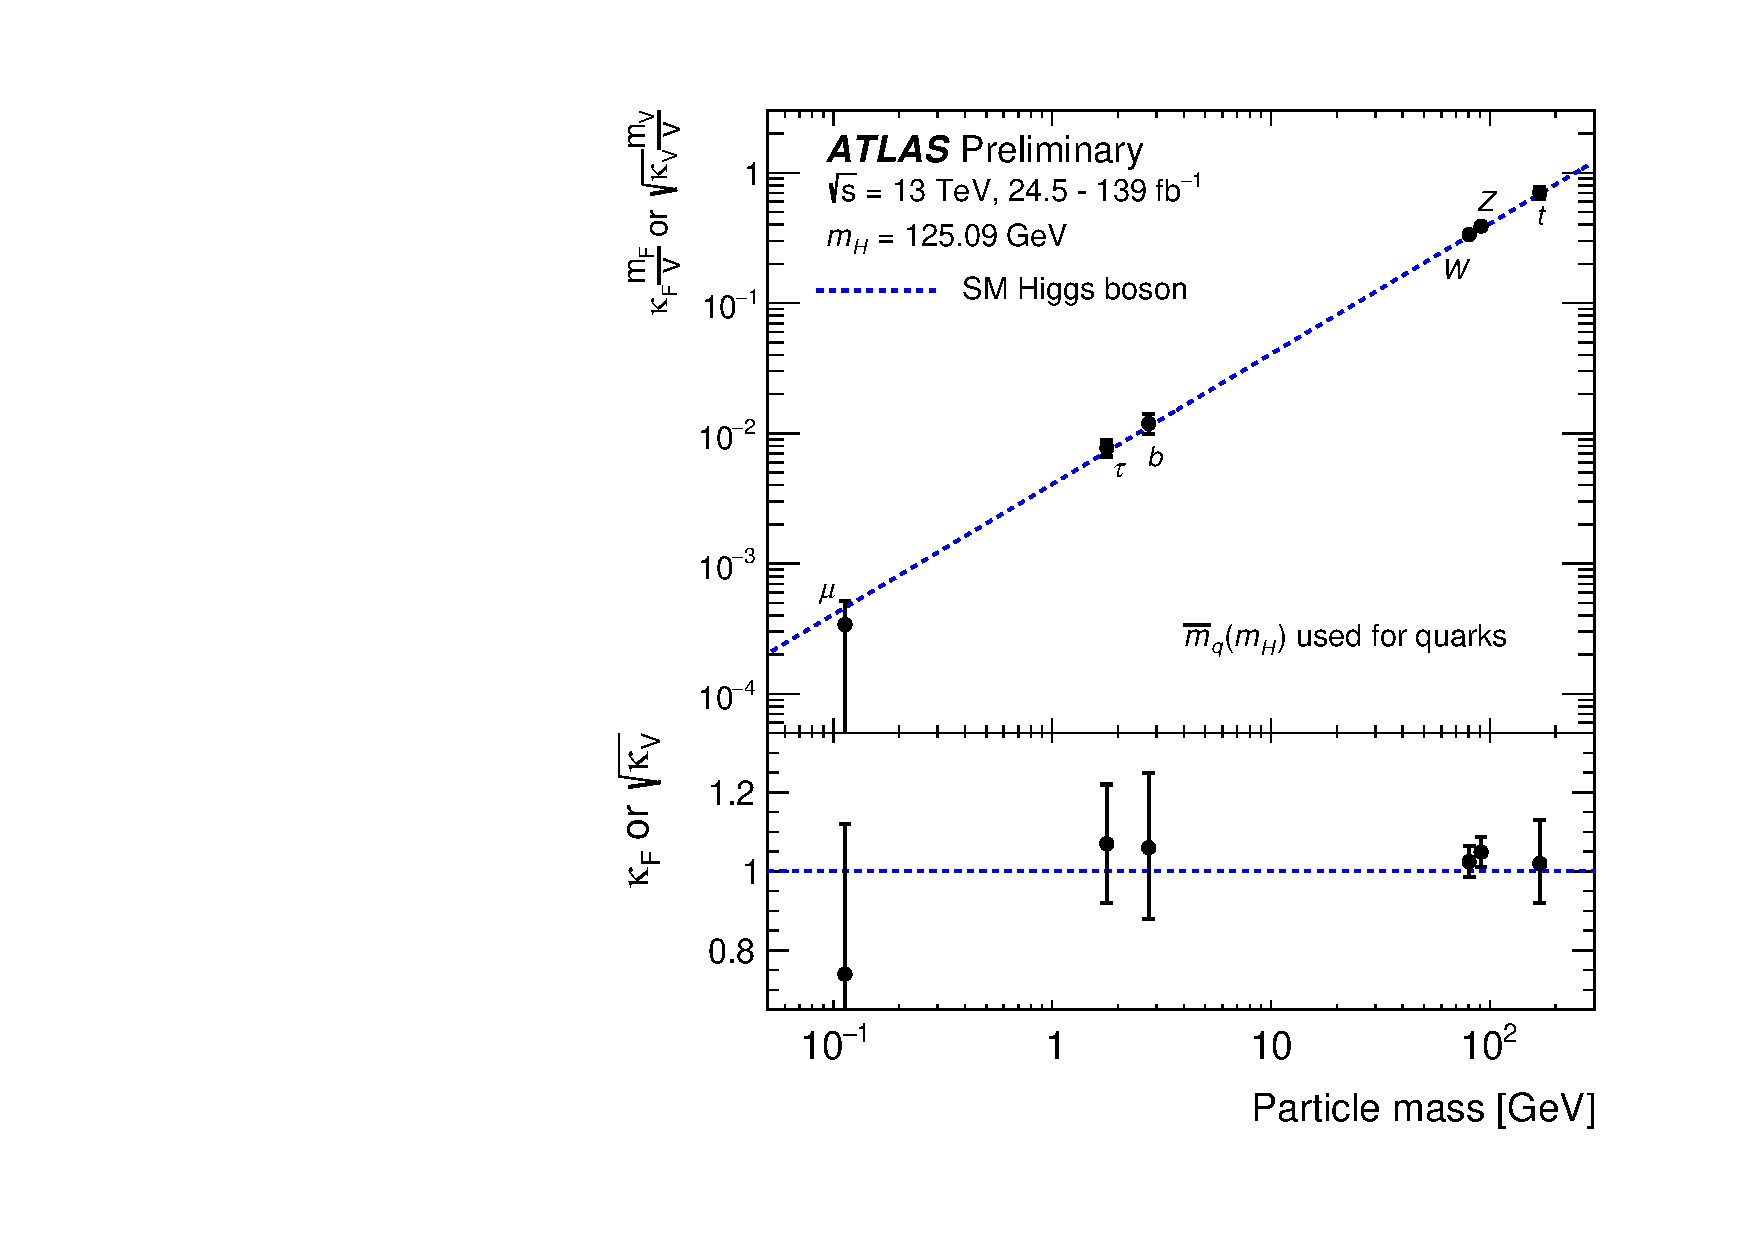
\includegraphics[width=0.49\textwidth]{figures/chapter1/sm_final/higgs_kappa_vs_mass}
        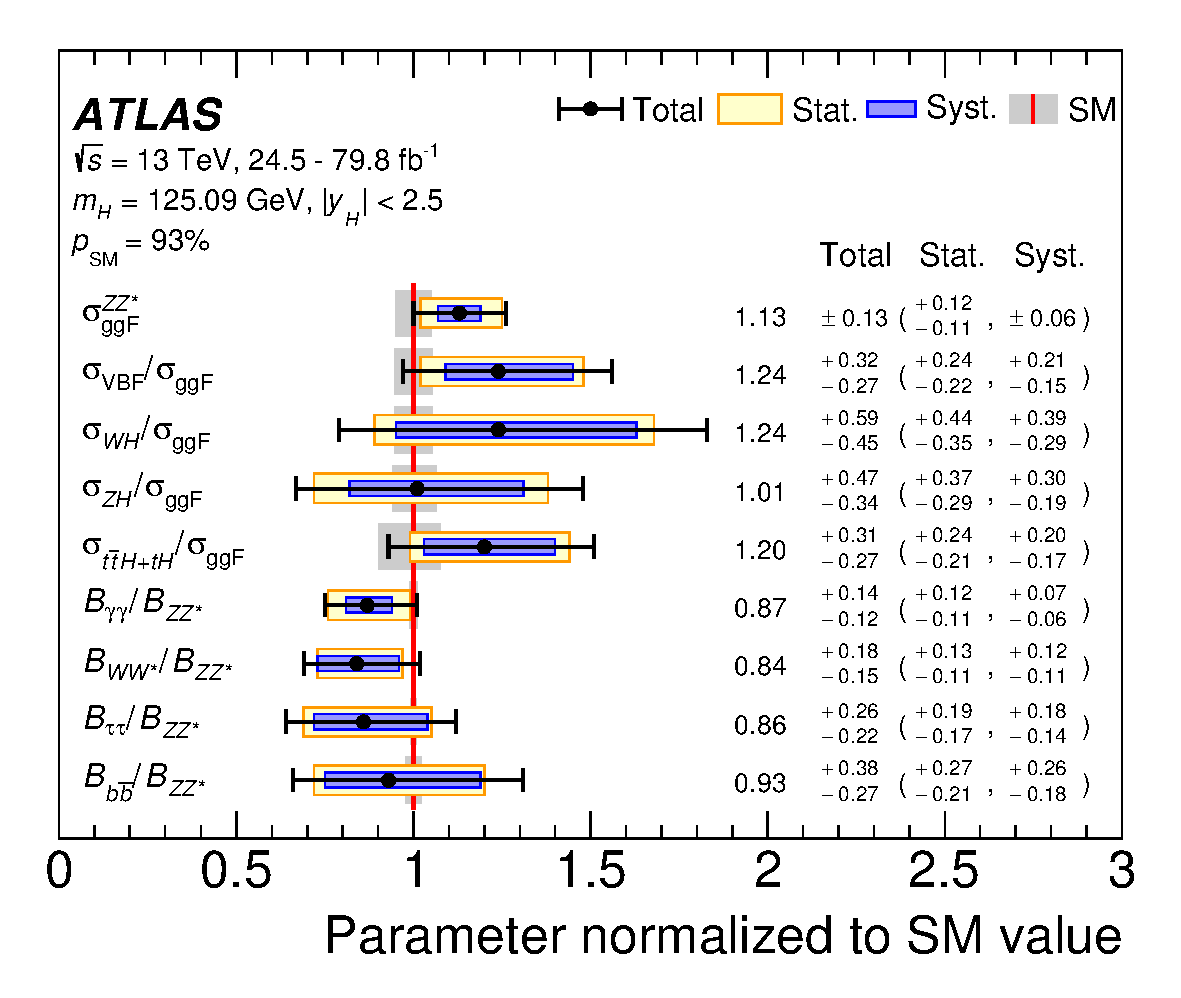
\includegraphics[width=0.49\textwidth]{figures/chapter1/sm_final/higgs_prod_and_br}
        \caption{
            Higgs precision measurements of couplings to SM particles.
            Figures from Ref.~\cite{HiggsProps}.
            \textit{\textbf{Left}}: Combined measurement of fermion and gauge-boson Higgs coupling modifiers, $\kappa_f$
                and $\kappa_V$ (assumed to be universal across fermion and gauge-boson species in the result pictured).
                Values of $\kappa_f$ or $\kappa_V$ equal to 1 correspond to the SM prediction for the Higgs' couplings to
                these particles.
            \textit{\textbf{Right}}: Measured values of the Higgs fermion and gauge-boson coupling parameters
                as a function of the fermion and gauge-boson masses.
                The blue dashed line shows the SM prediction (Equations~\ref{eq:higgs_gauge_couplings} and \ref{eq:higgs_fermion_coupling}).
            \textit{\textbf{Bottom}}: Measurements of Higgs production cross sections and (relative) decay branching ratios.
        }
        \label{fig:higgs_measurements}
    \end{center}
\end{figure}

In addition to the Higgs couplings to the SM fermions and gauge bosons, the SM Lagrangian
predicts terms describing the Higgs \textit{self}-couplings.
These terms are described by the $\lambda$ parameter in Equation~\ref{eq:higgs_potential}
and appearing in Table~\ref{tab:sm_content_EWSB}.
The Higgs self-coupling parameter $\lambda$ has a value predicted by the SM, as seen in 
Equation~\ref{eq:higgs_self_couplings}, which is fixed by the Higgs boson mass.
The parameter $\lambda$ is directly responsible for providing the structure of the Higgs potential,
indicated by Equation~\ref{eq:higgs_potential_self_int}, and therefore plays a fundamental
role in EWSB.
Measuring how the 125\,GeV Higgs boson couples and decays to the SM fermions and gauge bosons,
then, is only a necessary requirement for confirming that the particle is the one predicted by
the SM: it is not sufficient.
To truly confirm that the 125\,GeV boson is indeed that predicted by the SM, and that EWSB
is described by the BEH mechanism, the Higgs self-coupling parameter will have to be measured
experimentally and confirmed to take its predicted value given by Equation~\ref{eq:higgs_self_couplings}.

Direct measurement of $\lambda$ proceeds only through the observation of events in which Higgs bosons
are produced in pairs.
At the LHC, this process occurs predominantly via gluon-gluon fusion through the two diagrams illustrated
in Figure~\ref{fig:hh_feynman}.
The triangle and box diagrams shown in Figure~\ref{fig:hh_feynman} represent destructively interfering amplitudes.
As a result, the cross-sections associated with the production of Higgs boson pairs is exceedingly low
and statistically significant observation of this process is not expected to occur until
near the end of the lifetime of the LHC.
The study of Higgs boson pairs is the subject of the analysis to be presented in Chapter~\ref{chap:search_hh}.

\begin{figure}[!htb]
    \begin{center}
        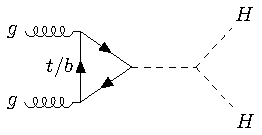
\includegraphics[width=0.7\textwidth]{figures/search_hh/feynman_diagrams/fdiagram_triangle}
        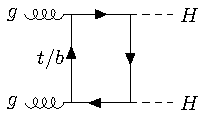
\includegraphics[width=0.55\textwidth]{figures/search_hh/feynman_diagrams/fdiagram_box}
        \caption{
            Representative Feynman diagrams that contribute at leading order in QCD to the non-resonant
            production of Higgs boson pairs.
            {\textbf{\textit{Top}}}: The `triangle' diagram, sensitive to the Higgs self-coupling, $\lambda$.
            {\textbf{\textit{Bottom}}}: The `box' diagram, sensitive to the (squared) Yukawa couplings to the third generation
            fermions entering the loop.
        }
        \label{fig:hh_feynman}
    \end{center}
\end{figure}

%%%%%%%%%%%%%%%%%%%%%%%%%%%%%%%%%%%%%%%%%%%%%%%%%%%%%%%%%%%%%%%%%%%%%%%%%%%%%%%%%
%%%%%%%%%%%%%%%%%%%%%%%%%%%%%%%%%%%%%%%%%%%%%%%%%%%%%%%%%%%%%%%%%%%%%%%%%%%%%%%%%
%%%%%%%%%%%%%%%%%%%%%%%%%%%%%%%%%%%%%%%%%%%%%%%%%%%%%%%%%%%%%%%%%%%%%%%%%%%%%%%%%
%
% SHORTCOMINGS
%
%%%%%%%%%%%%%%%%%%%%%%%%%%%%%%%%%%%%%%%%%%%%%%%%%%%%%%%%%%%%%%%%%%%%%%%%%%%%%%%%%
%%%%%%%%%%%%%%%%%%%%%%%%%%%%%%%%%%%%%%%%%%%%%%%%%%%%%%%%%%%%%%%%%%%%%%%%%%%%%%%%%
%%%%%%%%%%%%%%%%%%%%%%%%%%%%%%%%%%%%%%%%%%%%%%%%%%%%%%%%%%%%%%%%%%%%%%%%%%%%%%%%%
\FloatBarrier
\subsection{Perceived Shortcomings of the SM and Open Questions}
\label{sec:sm_shortcomings}

Despite the impressive results and predictive power of the SM illustrated in the previous
section, the SM is unable to provide a complete picture of what we now consider the observed
universe.
A few items that are clearly not explainable under the framework of the SM are described below.
Chapter~\ref{chap:bsm} goes on to introduce an extension to the SM that provides explanations
for many of these short comings of the SM.

\begin{description}
    \item[] \textbf{Existence of Dark Matter (DM) and Dark Energy (DE)} \\
        Most of the experimental evidence that we currently have that supports the notion that
        physics beyond the SM (BSM) exists comes not from collider-based particle physics experiments,
        but from astrophysical observations.
        Astrophysical observations suggest that the majority of the matter content of the universe
        is composed of a non-luminous, weakly interacting type of matter referred to as `Dark Matter' (DM)
        and that the expansion of the universe is accelerating, perhaps due to presence of
        `Dark Energy' (DE)~\cite{Davis:2014csa,PlanckCollab}.
        There has not yet been experimental proof of the particle nature of DM, but there
        many theories suggest that it fall under the class of `Weakly Interacting Massive Particle' (WIMPs) (`WIMP-like DM').
        The particle nature of DE is completely unknown and without a fundamental description.
    \item[] \textbf{Massive Neutrinos} \\ The observation of neutrino oscillations~\cite{Fukuda:1998mi} provides evidence
        in support neutrinos having nonzero masses, and contradicts the massless neutrino hypothesis of the SM.
    \item[] \textbf{Matter-Antimatter Asymmetry} \\
        The only parameter in the SM that allows for CP violation is the CP-violating phase in the CKM matrix,
        which is unable to account for the amount of CP violation needed to account for the
        observed asymmetry in the amount of matter over antimatter in the universe.
        Additional CP violating effects are necessary to account for this asymmetry and should be relevant
        to early universe cosmology~\cite{Sakharov_1991}.
    \item[] \textbf{The Hierarchy Problem} \\
        The Hierarchy Problem refers to the fact that the electroweak sector, through the scalar Higgs boson,
        is sensitive to high energy cut-off scales nearing the Planck Mass, $M_{P} \approx 10^{18}--10^{19}$\,GeV.
        This is evident when computing the higher-order corrections to the Higgs mass,
        \begin{align*}
            m_h^2 = m_{h,\,0}^2 + \Delta m_h^2,
        \end{align*}
        which are found to be quadratically divergent due to the fact that the Higgs is not protected by any fundamental
        internal symmetries:
        %\vspace{-1.2cm}
        \begin{align}
            \Delta m_h^2 = -\frac{ |y_f|^2 }{16 \pi^2} \left[ 2 \Lambda^2  + \mathcal{O} \left( m_f^2 \ln \left( \frac{\Lambda}{m_f} \right) \right) \right],
        \end{align}
        where $y_f$ is the fermion Yukawa coupling, $m_f$ is the associated fermion mass, and $\Lambda$ is the
        ultra-violate cut-off scale.
        Similar terms also appear for the SM gauge bosons, but given the near-unity Yukawa coupling of the top-quark,
        the divergence is most sensitive to the fermion terms appearing in the above via $y_t$.
        The apparent fact that the electroweak scale at which the Higgs boson is experimentally known to exist
        should be unavoidably sensitive to $M_P$, attempting to drive the Higgs boson mass to values 16 orders
        of magnitude larger than the measured one,
        is at the heart of the Hierarchy Problem.
        The high energy scales at which SM calculations fail are typically assumed to be the scales
        at which new physics arise and take over as a more complete description of high energy pheneomena.
        That the Higgs boson is apparently driven to these scales motivates the arguments in favor
        of their being new physics at or near the electroweak scale which cancel the quadratically
        divergent terms appearing in the Higgs mass corrections.
        That cancellations of terms on the order of $10^{30}$ ($\Lambda^2$) should be possible introduces the
        philosophical concerns of \textit{naturalness}, which ponder whether or not Nature is such
        that the additional sources of high energy physics --- not accounted for by the SM --- can conspire in such a way as to
        allow for such apparently perfectly-tuned cancellation.
\end{description}

%eq:higgs_potential
